% Chapter 5 -- Out-of-Sample Design and Forecast Evaluation
% Requires: amsmath, amssymb, booktabs, array, tabularx, graphicx, tcolorbox (breakable, skins), hyperref or url.
% Defines the callout box only if the preamble has not.
\providecolor{fenavy}{HTML}{1B2A6B}
\providecolor{feshade}{HTML}{F3F5FA}
\makeatletter
\@ifundefined{callout}{%
  \newtcolorbox{callout}{breakable, enhanced,
    colback=white, colframe=gray!70, boxrule=0.5pt, arc=1mm,
    borderline west={2.5pt}{0pt}{gray!70},
    left=8pt, right=8pt, top=4pt, bottom=4pt}%
}{}
\makeatother

\chapter{Out-of-Sample Design and Forecast Evaluation}
\label{ch:05}

Chapter 4 asked how strong the evidence must be when many strategies are tried. This chapter asks a different question about a single model: does it forecast, or did it only fit?

A regression estimated on the whole history of the data has seen every observation it is judged on. Its $R^2$ measures how well it describes the past, with the benefit of hindsight about which way the coefficients should point and how large they should be. A forecaster has no such benefit. At each date she knows only what had happened up to then, must estimate her model from that, and is judged on what happens next.

The claim on trial is one that most empirical finance took for granted until the mid-2000s: \textbf{a predictor that fits well in-sample will forecast well out of sample.}

By the end of the chapter you will be able to:

\begin{itemize}
  \item explain point forecasts, loss functions and information sets, and measure accuracy with the mean squared error;
  \item explain the bias--variance trade-off and why simple models often forecast better than rich ones;
  \item distinguish training, validation and test data, and explain why time series must be split in order;
  \item describe autoregressive models and persistence, and explain why in-sample $R^2$ flatters complex models;
  \item design a walk-forward evaluation that uses only information available at each forecast date, with expanding or rolling windows;
  \item recognize and remove the common forms of leakage, including the overlapping-target leak that purging and embargoing prevent;
  \item choose a benchmark that is hard to beat, and measure performance against it with the out-of-sample $R^2$ and the Clark--West and Diebold--Mariano tests;
  \item judge forecasts by their economic value and, for probabilistic forecasts, with proper scoring rules;
  \item explain why a predictor that truly works can still fail out of sample, and why one that fails can still be real.
\end{itemize}

In the lab you will take 14 variables that published research has used to predict the U.S. stock market, the data set of Goyal and Welch (2008), and ask each to forecast month by month from 1965 using only what was known at the time. A simulation in which the truth is known then shows how often each test reaches the right verdict.

\section{Foundations: the basics of forecasting}
\label{sec:05-foundations}

\textbf{Point forecasts and loss functions.} A \textbf{point forecast} is a single number: the forecaster's best guess of next month's return. ``Best'' depends on a \textbf{loss function} that says how costly each error is.

\begin{itemize}
  \item Under \textbf{squared-error loss}, an error of 2 costs four times as much as an error of 1. The best forecast is then the \textbf{conditional mean}, the average outcome given everything known at the time. Accuracy is measured by the \textbf{mean squared error} (MSE), the average of the squared forecast errors, or its square root (RMSE), which is in the same units as the forecast.
  \item Under absolute-error loss, an error of 2 costs twice as much as an error of 1, and the best forecast is the median.
\end{itemize}

Finance mostly uses squared error, because it connects directly to variance and to mean--variance portfolio choice.

\textbf{Information sets.} A forecast made at time $t$ may use only the \textbf{information set} available at $t$: past prices, published data, and models estimated on past observations. Everything in this chapter follows from enforcing that rule.

\textbf{The bias--variance trade-off.} A forecast's expected squared error has three parts (Figure~\ref{fig:05-biasvar}):

\begin{itemize}
  \item the irreducible \textbf{noise} in the outcome, which no model can remove;
  \item the \textbf{bias} from a model that is systematically wrong, for example because it leaves out a real effect;
  \item the \textbf{variance} from estimating the model on a finite sample: a different sample would give different coefficients and different forecasts.
\end{itemize}

Richer models, with more parameters, reduce bias but increase variance. When the signal is weak relative to the noise, as for stock returns, a simple model with few parameters often forecasts better than a rich one, even if the rich one is closer to the truth. Fitting the noise in a sample instead of the signal is called \textbf{overfitting}.

\providecolor{fenavy}{HTML}{1B2A6B}
\providecolor{fegray}{HTML}{4D4D4D}

\begin{figure}[htbp]
  \centering
  \begin{tikzpicture}[
    declare function={
      bias(\x)  = 0.67/(\x + 0.47);   % squared bias: falls with complexity
      var(\x)   = 0.0048*\x^2.16;     % variance: rises with complexity
      noise     = 0.14;               % irreducible noise
    }]
  \begin{axis}[
    width=0.85\linewidth, height=0.52\linewidth,
    axis lines=left,
    axis line style={-stealth, thin},
    xmin=0, xmax=10.3, ymin=0, ymax=1.08,
    xtick=\empty, ytick=\empty,
    xlabel={Model complexity (number of parameters)},
    ylabel={Expected forecast error},
    samples=200,
    clip=false,
  ]
    % Components
    \addplot[fegray, thick, dashed, domain=0.24:10] {bias(x)};
    \addplot[fegray, thick, densely dotted, domain=0:10] {var(x)};
    \addplot[gray, thin, domain=0:10] {noise};
    % Total = bias + variance + noise
    \addplot[fenavy, very thick, domain=0.27:10] {bias(x) + var(x) + noise};

    % Best point
    \draw[fenavy, densely dashed, thin] (axis cs:3.45,0) -- (axis cs:3.45,0.381);
    \node[fenavy, anchor=south] at (axis cs:3.45,0.47) {best};

    % Right-hand labels
    \node[fenavy, anchor=west] at (axis cs:10.1,0.898) {total error};
    \node[fegray, anchor=west] at (axis cs:10.1,0.694) {variance};
    \node[gray,   anchor=west] at (axis cs:10.1,0.16)  {noise};
    \node[fegray, anchor=west] at (axis cs:10.1,0.05) {bias};

    % Regions
    \node[anchor=west] at (axis cs:0.6,1.0)  {underfit};
    \node[anchor=west] at (axis cs:7.3,0.53) {overfit};
  \end{axis}
  \end{tikzpicture}
  \caption{The bias--variance trade-off. Adding parameters lowers bias but
    raises the variance that comes from estimating them. Total forecast error
    is lowest at an intermediate complexity. When the signal is weak, as for
    stock returns, the best point lies far to the left.}
  \label{fig:05-biasvar}
\end{figure}

%\begin{figure}[htbp]
%\centering
%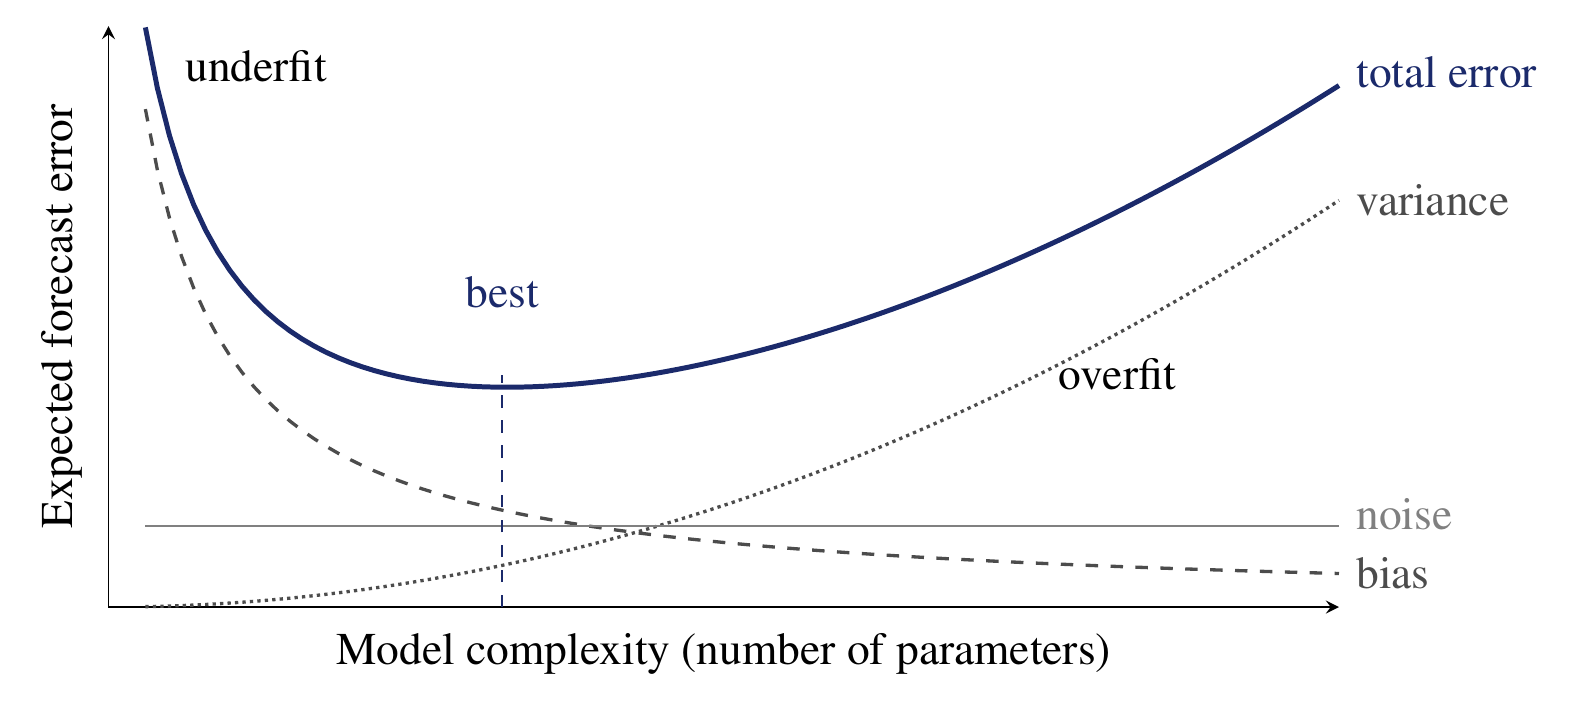
\includegraphics[width=0.85\linewidth]{images/fig05-1-bias-variance.png}
%\caption{The bias--variance trade-off. Adding parameters lowers bias but raises the variance that comes from estimating them. Total forecast error is lowest at an intermediate complexity. When the signal is weak, as for stock returns, the best point lies far to the left.}
%\label{fig:05-biasvar}
%\end{figure}

\textbf{Training, validation and test data.} Machine learning separates data into three parts:

\begin{itemize}
  \item a \textbf{training set} to estimate the model;
  \item a \textbf{validation set} to choose among models or tune settings;
  \item a \textbf{test set}, used once, to measure performance.
\end{itemize}

In time series the order matters: the training data must come before the test data, so random splits used for independent observations are not valid.

\textbf{Autoregressive models.} The simplest time-series forecasting model predicts a variable from its own past. The \textbf{first-order autoregressive model}, AR(1), is
\begin{equation}
  y_{t+1} = c + \phi\,y_t + \varepsilon_{t+1}
  \label{eq:05-ar1}
\end{equation}
The parameter $\phi$ measures \textbf{persistence}: values near 1 mean the series moves slowly, like interest rates or valuation ratios; values near 0 mean it is close to unpredictable, like stock returns. A \textbf{predictive regression} replaces $y_t$ on the right with another variable $x_t$ believed to carry information about $y_{t+1}$.

\textbf{In-sample $R^2$.} For a regression estimated on the data it is judged on,
\begin{equation}
  R^2 = 1 - \frac{\text{sum of squared residuals}}{\text{total sum of squares}}
  \label{eq:05-r2}
\end{equation}
where the total sum of squares measures how far the outcomes vary around their own mean. This $R^2$ can never be negative, and adding variables can never reduce it. This is why in-sample fit flatters complex models.

\textbf{Worked example.} A model with an in-sample $R^2$ of 2\% on monthly returns explains 2\% of the variance of returns. If returns have a monthly standard deviation of 4.5\%, the model's forecasts vary with a standard deviation of only about $\sqrt{0.02} \times 4.5\% \approx 0.6\%$ a month, small next to the noise in any single month.

\textbf{Further reading.} Hyndman and Athanasopoulos, \emph{Forecasting: Principles and Practice} (free online), chapters on forecast evaluation and time-series cross-validation; Diebold, \emph{Forecasting in Economics, Business, Finance and Beyond} (free online); Hastie, Tibshirani and Friedman, \emph{The Elements of Statistical Learning}, chapter on model assessment and selection.

\section{In-sample fit versus out-of-sample performance}
\label{sec:05-insample}

The standard test of return predictability is a regression of next period's excess return on a variable known today:
\begin{equation}
  r_{t+1} = \alpha + \beta x_t + \varepsilon_{t+1}
  \label{eq:05-pred}
\end{equation}

If $\beta$ is significantly different from zero, $x$ is said to predict returns. Fama and French (1988) and Campbell and Shiller (1988) used regressions like this to argue that the dividend--price ratio predicts stock returns, and dozens of other variables followed: interest rates, yield spreads, inflation, the volume of share issuance, measures of risk. By the early 2000s, predictability of the equity premium was widely regarded as a stylized fact.

Goyal and Welch (2008) asked a simple question of these predictors. Suppose an investor in 1965 had used each one, estimating the regression with data only up to the forecast date and re-estimating it every month. Would she have forecast better than someone who simply used the average past return? For most predictors the answer was no. Many that were significant in-sample produced out-of-sample forecasts worse than the historical mean, and the few that helped did so only in some decades. Their 2024 update with Zafirov found the same pattern for predictors proposed since.

Three forces open the gap between fit and forecast.

\textbf{Estimation error.} A forecaster must estimate $\alpha$ and $\beta$ from a finite sample, and the errors in those estimates become errors in her forecasts. When the true predictable share of returns is tiny, as it is for monthly stock returns, this noise can outweigh the signal. As a rough guide, estimating one extra slope from $n$ months of data costs about $1/n$ of $R^2$: with 40 years of monthly data, $n = 480$, about 0.2\%. The best equity-premium predictors are thought to explain perhaps 0.5\% to 1\% of monthly variation. The margin is thin.

\textbf{Instability.} Relationships in markets change. A predictor may work in one era and not another because the economy changes, because investors learn, or because the predictor itself was an artifact of one period. An in-sample regression averages over all eras; a forecaster lives through them in order.

\textbf{Selection.} Chapter 4's problem returns in a quieter form. Predictors that appear in the literature were selected partly because they fit the data their discoverers had. That fit is partly luck, and luck does not repeat.

A fourth problem inflates in-sample evidence itself. Most popular predictors, such as valuation ratios and interest rates, are highly persistent, and their surprises are correlated with return surprises. Stambaugh (1999) showed that this biases the estimated slope in finite samples and makes conventional t-statistics too large. Chapter 3's lab demonstrated the related problem of overlapping long-horizon regressions.

\textbf{Out-of-sample tests are not automatically better.} Inoue and Kilian (2004) pointed out that in-sample tests are more powerful: they use all the data to estimate the parameters, while out-of-sample tests spend part of the sample on training. A predictor can be genuine and still fail out of sample because the test lacks power. The value of out-of-sample evaluation is not that it is more accurate in theory, but that it is harder to fool: it guards against data mining, against hindsight in the choice of specification, and against relationships that have broken down. This chapter's lab measures both sides of that trade-off.

\section{Walk-forward evaluation: expanding and rolling windows}
\label{sec:05-walkforward}

A \textbf{walk-forward} (or recursive) evaluation replays history as a forecaster would have lived it:

\begin{enumerate}
  \item Choose a first forecast date, leaving enough earlier data to estimate the model.
  \item Estimate the model using only data available at that date.
  \item Forecast the next period, and record the forecast and the benchmark's forecast.
  \item Move forward one period, add the new observation, and repeat.
\end{enumerate}

The result is a series of genuine forecasts, each made without knowledge of what followed. Evaluation statistics are computed on this series alone.

The main design choice is which past data to use at each step (Figure~\ref{fig:05-windows}):

\begin{center}
\small
\begin{tabularx}{0.9\linewidth}{@{}>{\raggedright\arraybackslash}p{0.13\linewidth}>{\raggedright\arraybackslash}X>{\raggedright\arraybackslash}p{0.24\linewidth}>{\raggedright\arraybackslash}p{0.24\linewidth}@{}}
\toprule
Window & Training data at each date & Strength & Weakness \\
\midrule
Expanding & All data from the start of the sample & Most data, lowest estimation error & Slow to adapt if the relationship changes \\
Rolling & The most recent $w$ periods only & Adapts to change & More estimation error; results depend on $w$ \\
Fixed & One training period, never updated & Simplest; mimics a model frozen at launch & Ignores new information \\
\bottomrule
\end{tabularx}
\end{center}

\providecolor{fenavy}{HTML}{1B2A6B}

\begin{figure}[htbp]
  \centering
  \begin{tikzpicture}[
    x=0.36cm, y=0.5cm,
    est/.style={fill=fenavy!18, draw=white, line width=0.6pt},
    fc/.style={fill=fenavy, draw=white, line width=0.6pt},
    lab/.style={anchor=east, font=\small},
    head/.style={anchor=west, font=\small\bfseries},
  ]
    \def\wfOff{16}  % horizontal start of the right-hand panel

    % ---------- Expanding window (left) ----------
    \node[head] at (0,1.2) {Expanding window};
    \foreach \wfS in {1,...,5} {
      \pgfmathsetmacro{\wfY}{-\wfS+1}
      \node[lab] at (-0.3,\wfY) {Step \wfS};
      \fill[est] (0,\wfY-0.3) rectangle (8+\wfS,\wfY+0.3);
      \fill[fc]  (8+\wfS,\wfY-0.3) rectangle (9+\wfS,\wfY+0.3);
    }

    % ---------- Rolling window (right) ----------
    \node[head] at (\wfOff,1.2) {Rolling window};
    \foreach \wfS in {1,...,5} {
      \pgfmathsetmacro{\wfY}{-\wfS+1}
      \fill[est] (\wfOff+\wfS-1,\wfY-0.3) rectangle (\wfOff+8+\wfS,\wfY+0.3);
      \fill[fc]  (\wfOff+8+\wfS,\wfY-0.3) rectangle (\wfOff+9+\wfS,\wfY+0.3);
    }

    % Time axis under both panels
    \draw[-stealth, thin] (0,-5) -- (\wfOff+15.2,-5)
      node[anchor=west, font=\small] {time};

    % Legend
    \fill[est] (4,-6.35) rectangle (5.5,-5.65);
    \node[anchor=west, font=\small] at (5.8,-6) {training data};
    \fill[fc]  (\wfOff,-6.35) rectangle (\wfOff+1.5,-5.65);
    \node[anchor=west, font=\small] at (\wfOff+1.8,-6) {forecast period};
  \end{tikzpicture}
  \caption{Walk-forward evaluation. At each step the model is estimated on the
    light bar and forecasts the dark one; then the evaluation moves forward one
    period. An expanding window keeps all past data; a rolling window keeps a
    fixed length and drops the oldest observations.}
  \label{fig:05-windows}
\end{figure}

%\begin{figure}[htbp]
%\centering
%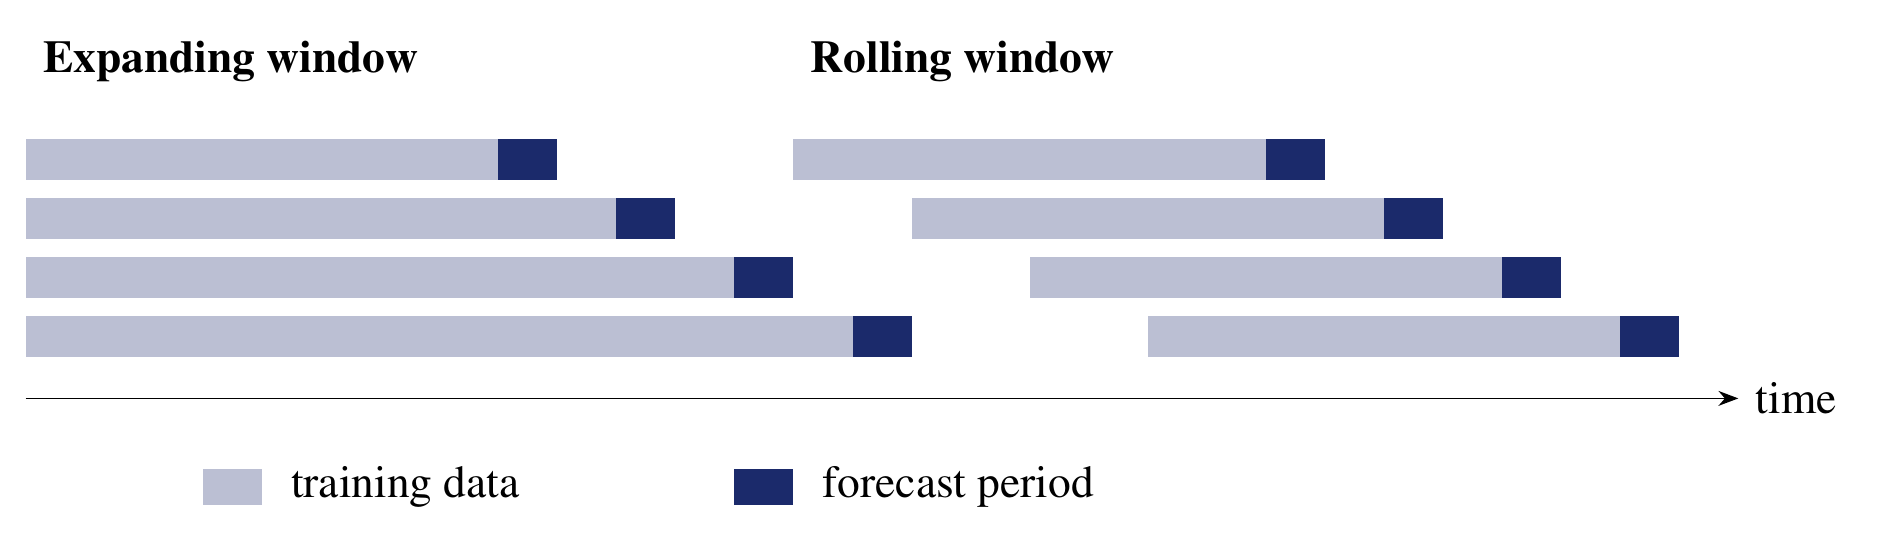
\includegraphics[width=0.9\linewidth]{images/fig05-2-walk-forward.png}
%\caption{Walk-forward evaluation. At each step the model is estimated on the light bar and forecasts the dark one; then the evaluation moves forward one period. An expanding window keeps all past data; a rolling window keeps a fixed length and drops the oldest observations.}
%\label{fig:05-windows}
%\end{figure}

No window is right in general. The choice is a bet on whether the relationship is stable (favoring expanding windows) or changing (favoring rolling ones). The danger is choosing the window after seeing which one works best: that is a search, and Chapter 4 applies. Decide the window, the first forecast date and the minimum training period before looking at the results, and report sensitivity to the alternatives.

\textbf{Restrictions from theory.} Campbell and Thompson (2008) showed that two simple restrictions, motivated by economics rather than statistics, improve many predictors' out-of-sample performance:

\begin{itemize}
  \item if the estimated slope has the opposite sign to the one theory predicts, use the historical mean instead;
  \item never forecast a negative equity premium, since investors would not hold stocks expecting to lose.
\end{itemize}

Restrictions like these reduce estimation error by ruling out implausible forecasts. They are legitimate if fixed in advance, and a form of search if chosen afterward.

\textbf{Re-estimation is part of the model.} In machine-learning applications the same logic covers every choice fitted to data: hyperparameters, \textbf{feature selection} (choosing which input variables to use), the choice among models. All must be redone inside each training window, using only that window's data. A model whose hyperparameters were tuned on the full sample has seen the test data, however carefully its coefficients were estimated.

\section{Leakage: look-ahead, publication lags, purging and embargoing}
\label{sec:05-leakage}

\textbf{Leakage} is any route by which information from the test period reaches the model or the evaluation. It is the most common reason a backtest looks better than live trading, and it rarely announces itself. The forms worth checking for are these.

\textbf{Full-sample estimation.} The classic error is to estimate a model on the whole sample and then ``test'' it on part of the same sample. The coefficients already know how the test period turned out. The same applies to anything fitted: standardizing variables with full-sample means and standard deviations, choosing lags, or \textbf{winsorizing}, capping extreme values at chosen percentiles, when those percentiles come from the full sample.

\textbf{Hindsight in choosing the model.} Choosing which predictor to use, or which of several models, because it performed well over the whole sample is look-ahead even if each model is then evaluated walk-forward. The honest version makes the choice at each date using only past data.

\textbf{Publication lags and revisions.} A variable dated March is not necessarily known in March. Consumer prices for March are published in April; company earnings for a quarter arrive weeks or months later; many macroeconomic series are revised for years after first release. Using the final, revised value as if it had been known on its reference date is leakage. Goyal and Welch lag inflation by an extra month for this reason. For macroeconomic predictors, real-time vintages such as the Federal Reserve Bank of St.\ Louis's ALFRED archive record what was known when. Chapter 2's discussion of point-in-time data (Section~\ref{sec:02-lookahead}) applies throughout.

\textbf{Overlapping targets.} Suppose the target is the return over the next 12 months. The observation formed in June has a target that runs through the following June. If the model is trained at the end of December on all observations up to November, the last eleven of them have targets that include returns after December, which the forecaster could not have known. A walk-forward evaluation must therefore drop those observations from training (Figure~\ref{fig:05-purging}). L\'opez de Prado (2018) calls this \textbf{purging}: removing from the training set every observation whose target overlaps the test period.

\providecolor{fenavy}{HTML}{1B2A6B}

\begin{figure}[htbp]
  \centering
  \begin{tikzpicture}[
    x=0.28cm, y=0.42cm,
    lab/.style={anchor=west, font=\small, align=left},
  ]
    % Months relative to the forecast date (0). Each observation is formed at
    % month m and paired with the 12-month return from m to m+12.

    % Kept: target ends before the forecast date
    \foreach \wfM [count=\wfR from 0] in {-17,-15,-13} {
      \draw[fenavy, thick] (\wfM,\wfR) -- (\wfM+12,\wfR);
      \fill[fenavy] (\wfM,\wfR) circle (2.6pt);
    }

    % Purged: target runs past the forecast date
    \foreach \wfM [count=\wfR from 3] in {-11,-9,-7,-5,-3,-1} {
      \draw[gray!55, densely dashed] (\wfM,\wfR) -- (\wfM+12,\wfR);
      \fill[gray!55] (\wfM,\wfR) circle (2.6pt);
    }

    % Forecast date
    \draw[fenavy, thick] (0,-1.5) -- (0,8.6);
    \node[fenavy, font=\small, anchor=south, align=center] at (0,8.6)
      {forecast date\\(end of December)};

    % Time axis
    \draw[-stealth, thin] (-18.5,-1) -- (13,-1)
      node[anchor=west, font=\small] {months};

    % Labels
    \node[lab, gray] at (13.5,7) {purged: target runs\\past the forecast date};
    \node[lab, fenavy] at (1.2,0.7) {kept: 12-month target\\ends before the forecast};
    \node[font=\small, gray!40!black, anchor=north, align=center]
      at (-9,-1.6) {training observations (dot $=$ date formed;\\
                    line $=$ 12-month return it is trained to predict)};
  \end{tikzpicture}
  \caption{Purging. Each training observation is paired with the 12-month
    return that follows it. Observations whose 12-month target runs past the
    forecast date (dashed) contain returns the forecaster could not yet know,
    so they are removed from the training set.}
  \label{fig:05-purging}
\end{figure}

%\begin{figure}[htbp]
%\centering
%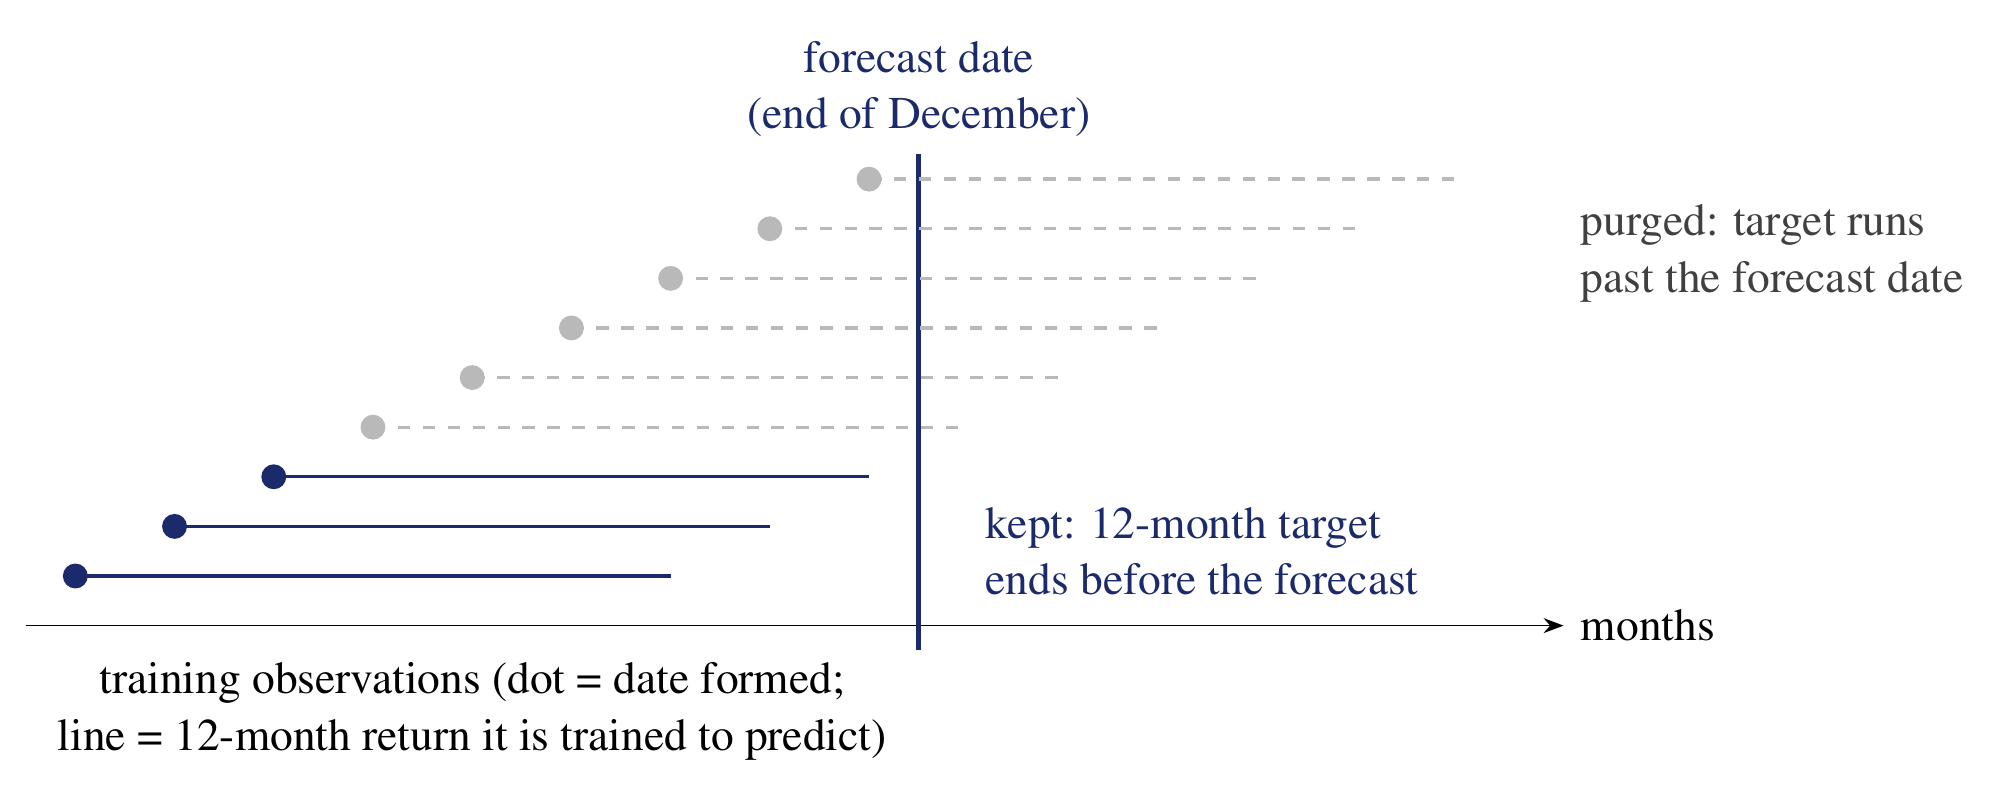
\includegraphics[width=0.85\linewidth]{images/fig05-3-purging.png}
%\caption{Purging. Each training observation is paired with the 12-month return that follows it. Observations whose 12-month target runs past the forecast date (dashed) contain returns the forecaster could not yet know, so they are removed from the training set.}
%\label{fig:05-purging}
%\end{figure}

\textbf{Serial correlation across the boundary.} When training data can come after the test period, as in the cross-validation of Chapter 4, observations just after the test period may still carry information about it through serially correlated features. L\'opez de Prado's \textbf{embargo} drops a short period of training data immediately after each test block. In a pure walk-forward design, where training always precedes testing, purging is needed but an embargo is not.

\textbf{Survivorship and selection in the data.} Datasets of current index members, surviving funds or listed firms build in knowledge of who survived. Chapter 2 covered these traps; they matter as much for forecasting as for backtesting.

Lab 5 measures several of these leaks on real data, comparing each with its honest counterpart.

\section{Benchmarks that are hard to beat}
\label{sec:05-benchmarks}

A forecast is only as impressive as the alternative it beats. Choosing a weak benchmark, such as zero, or a model nobody would use, is one of the easiest ways to make a forecasting method look good. The benchmarks that matter are the simple ones a sensible person would use without any model at all.

\begin{center}
\small
\begin{tabularx}{0.9\linewidth}{@{}>{\raggedright\arraybackslash}p{0.18\linewidth}>{\raggedright\arraybackslash}p{0.28\linewidth}>{\raggedright\arraybackslash}X@{}}
\toprule
Quantity forecast & Natural benchmark & Why it is hard to beat \\
\midrule
Equity premium & Historical mean of past returns & Only one parameter to estimate; no exposure to unstable relationships \\
Exchange rates, asset prices & Random walk: tomorrow equals today & Meese and Rogoff (1983) found that structural exchange-rate models did not beat it, a result that has proved durable \\
Interest rates, yields & Random walk, or the forward rate & Rates are highly persistent; Chapter 16 tests the forward rate as a forecast \\
Volatility & Recent realized volatility, or a simple exponentially weighted average & Volatility clusters, so the recent past is informative; Chapter 11 tests richer models \\
Macroeconomic series & Survey consensus, or the last value & Professional forecasters already use most public information \\
\bottomrule
\end{tabularx}
\end{center}

An \textbf{exponentially weighted average} gives the most weight to the latest observation and steadily less to older ones. A \textbf{survey consensus} is the average forecast of professional forecasters.

The historical mean is the benchmark for the equity premium because it is what an investor would assume without a forecasting model. It is computed in real time, with the same training data as the model, so that the comparison isolates the value of the predictor. Beating it is hard for the reason given in Section~\ref{sec:05-insample}: the predictor's signal is small and its estimation error is not.

A useful habit is to name the benchmark before building the model, and to ask what a skeptical colleague would accept as the default. If a new method cannot beat that default, its sophistication is a cost rather than a benefit.

\section{Measuring forecast accuracy: out-of-sample $R^2$, Diebold--Mariano and Clark--West}
\label{sec:05-accuracy}

\textbf{The out-of-sample $R^2$.} Campbell and Thompson (2008) summarized forecast accuracy against the historical mean with
\begin{equation}
  R^2_{OS} = 1 - \frac{\sum_t (r_{t+1} - \hat r_{t+1})^2}{\sum_t (r_{t+1} - \bar r_{t})^2}
  \label{eq:05-r2os}
\end{equation}
where $\hat r_{t+1}$ is the model's forecast and $\bar r_t$ the historical mean, both computed from data up to $t$. Unlike the in-sample $R^2$ of Equation~\eqref{eq:05-r2}, it can be negative, and it is negative whenever the model's squared errors exceed the benchmark's. Positive values are small in this field. For monthly stock returns, an out-of-sample $R^2$ of 0.5\% would be a good result.

Goyal and Welch (2008) added a picture that is often more revealing than any summary statistic: the cumulative difference between the benchmark's squared errors and the model's, plotted over time. A line that rises steadily indicates a model that keeps winning; one that rises in a single episode and then drifts sideways or down indicates a result that depends on one period.

\textbf{Is the difference significant?} Diebold and Mariano (1995) proposed testing whether two forecasts are equally accurate by looking at the series of differences in their losses,
\begin{equation}
  d_t = e^2_{\text{bench},t} - e^2_{\text{model},t}
  \label{eq:05-dm}
\end{equation}
where $e$ denotes a forecast error. If the forecasts are equally accurate, $d_t$ has mean zero; a t-test on its mean, with Newey--West standard errors for multi-step forecasts (Section~\ref{sec:03-se}), gives the test. Harvey, Leybourne and Newbold (1997) proposed a small-sample correction that is now standard.

\textbf{The nested-model problem.} Two models are \textbf{nested} when one is a special case of the other. The DM test was designed for competing forecasts. When the model contains the benchmark as a special case, as a predictive regression contains the historical mean (set $\beta = 0$), the test misbehaves. Under the null that $\beta = 0$, the larger model still estimates $\beta$, and the estimation noise makes its forecasts slightly worse on average. The DM statistic is then centered below zero, and the test rejects too rarely. Clark and West (2007) proposed an adjustment that adds back the expected cost of that noise:
\begin{equation}
  f_t = (r_{t+1} - \bar r_t)^2 - \left[(r_{t+1} - \hat r_{t+1})^2 - (\bar r_t - \hat r_{t+1})^2\right]
  \label{eq:05-cw}
\end{equation}
and a one-sided t-test on the mean of $f_t$. It is the standard test for the equity-premium literature, and the lab reports it alongside DM. Note the asymmetry: Clark--West can declare a model significantly informative even when its out-of-sample $R^2$ is slightly negative, because it asks whether the predictor carries information, not whether this particular estimated forecast beat the mean.

\textbf{Economic value.} Statistical accuracy and economic value are not the same thing. Campbell and Thompson showed that an investor who times the market can gain substantially from an $R^2$ that looks negligible. Roughly, a market timer's expected excess return rises in proportion to $R^2/S^2$, where $S$ is the market's Sharpe ratio per period. With a monthly Sharpe ratio of about 0.12 (0.42 a year) and a monthly $R^2$ of 0.5\%, the ratio is $0.005/0.12^2 \approx 0.35$: the timer's expected excess return rises by about a third.

The lab measures economic value directly. A \textbf{mean--variance investor}, who cares only about the mean and variance of her portfolio's return, uses each forecast to set her equity weight, and the result is compared with the same investor using the historical mean. The difference is reported as a gain in \textbf{certainty-equivalent return}: the riskless return she would accept instead of the risky strategy. This translates a forecast into the unit an investor cares about, but it depends on the investor's \textbf{risk aversion}, how much expected return she demands per unit of variance, and on the limits placed on her weights, so those choices should also be fixed in advance.

\section{Probabilistic forecasts and proper scoring rules}
\label{sec:05-scoring}

Much of finance needs more than a single number. A risk manager needs the probability of a large loss; an option trader needs a distribution of future prices; a portfolio optimizer needs variances as well as means. Forecasts in these settings are \textbf{probabilistic}: a full predictive distribution rather than a point.

Judging a distribution against a single realized outcome requires a \textbf{scoring rule}, a function that assigns a score to a forecast distribution $F$ and an outcome $y$. A scoring rule is \textbf{proper} if a forecaster expects the best score by reporting her true beliefs, and strictly proper if only her true beliefs achieve it (Gneiting and Raftery 2007). Proper scores matter because improper ones reward distortion: a forecaster judged only on whether outcomes fall inside her 90\% intervals, for example, can score perfectly by making the intervals enormous.

Two proper scores dominate practice:

\begin{itemize}
  \item \textbf{The log score}, $\log f(y)$, the log of the predicted \textbf{density}, the height of the forecast distribution, at the realized outcome. It rewards putting high probability where outcomes occur and punishes severely any outcome given near-zero probability. It is the natural score for likelihood-based models and is closely linked to information theory. Higher is better.
  \item \textbf{The continuous ranked probability score (CRPS)}, the integrated squared difference between the forecast distribution function and a step function that jumps from 0 to 1 at the outcome. It is measured in the units of the variable, reduces to absolute error for a point forecast, and is more forgiving of occasional extreme outcomes than the log score. Lower is better.
\end{itemize}

\textbf{Calibration} checks complement scores. A forecaster is calibrated if her stated probabilities match how often things happen: her 90\% intervals should contain the outcome about 90\% of the time. A related check uses the \textbf{probability integral transform}: if each outcome $y$ is converted to $F(y)$, its percentile under the forecast distribution, these values should be spread evenly between 0 and 1. Calibration is necessary but not sufficient: the historical distribution of returns, issued every day, is calibrated over the long run and still useless for timing. A good probabilistic forecast is calibrated and \textbf{sharp}, concentrating probability as tightly as calibration allows.

The same evaluation logic applies as for point forecasts. Scores must come from walk-forward forecasts; differences in average scores between a model and a benchmark can be tested with a Diebold--Mariano-type statistic; and the benchmark should be hard to beat. For return distributions, a normal distribution with the historical mean and recent volatility is a sensible default. The lab compares log scores and CRPS for each predictor against that benchmark, holding volatility fixed so that only the forecast mean differs. Chapters 11 and 13 return to probabilistic forecasts of volatility and of tail losses.

\section{Post-publication samples as natural experiments}
\label{sec:05-postpub}

Every walk-forward evaluation on historical data has a weakness: the researcher designing it knows roughly how history turned out. She knows the 1970s brought inflation, the 1990s a bull market and 2008 a crisis, and that knowledge can shape choices of predictors, windows and sample periods without her noticing.

The cleanest out-of-sample test uses data that did not exist when the idea was proposed. Once a predictor or anomaly is published, the years that follow are a test its authors could not have fitted: a \textbf{natural experiment}, in which the world rather than the researcher supplies the test. McLean and Pontiff (2016) used this logic for 97 cross-sectional anomalies: returns were 26\% lower in the period between the end of each original sample and publication, and 58\% lower after publication. They read the first decline as an upper bound on the effect of data mining, and the remainder as the effect of investors trading on the published result. Chapter 10 tests their findings in detail.

The same test applies to predictors of the market as a whole. The lab splits each predictor's out-of-sample forecasts at the year of an early paper proposing it and compares the two periods. The comparison is noisy, and publication years are a blunt marker of when an idea became known, but the direction of the difference is informative. Post-publication data has two further limits: it accumulates slowly, and a decline after publication can reflect a changed market as well as an overfit original result. It is the strongest out-of-sample evidence available, not a perfect experiment.

\begin{callout}
\textbf{What Failed: the dividend yield.} The dividend--price ratio is the most studied predictor of the stock market. Through the 1980s its in-sample record looked strong: when dividends were high relative to prices, subsequent returns were high (Fama and French 1988; Campbell and Shiller 1988). Then, through the 1990s, the ratio fell to the lowest levels in its history, signaling poor returns year after year, while stocks rose strongly. A forecaster using it in real time would have stayed underweight equities through one of the great bull markets. Goyal and Welch (2008) found that the dividend--price ratio and most other predictors did not beat the historical mean out of sample, and that much of their in-sample significance came from a few episodes, notably the oil shock of 1973--75. The debate did not end there. Cochrane (2008) argued that predictability is implied by the fact that dividend growth is not predictable, and Lettau and Van Nieuwerburgh (2008) that shifts in the ratio's long-run mean explain much of the failure. Chapter 7 puts the broader claim that stock returns are predictable on trial. The lesson for this chapter is about method: a relationship that held across a sample can fail for the person who must use it in real time. For that person, the verdict on the claim that the dividend yield forecasts returns is \textbf{weakens}: the economic logic is sound, but as a real-time forecasting tool it has not delivered.
\end{callout}

\section{Lab 5: Does it forecast, or did it fit?}
\label{sec:05-lab}

\begin{callout}
\textbf{Lab 5 at a glance.} \emph{Claim on trial:} a predictor that fits well in-sample will forecast well out of sample. \emph{Data:} the monthly predictor data that Amit Goyal publishes for Goyal and Welch (2008), updated through 2025. \emph{Run time:} under a minute. \emph{Code:} repository folder \texttt{ch05-forecasting/}, with a guided notebook.
\end{callout}

The lab applies every tool in this chapter to the most studied forecasting problem in finance. Chapter 7 uses the same data to judge whether returns are predictable; this lab is about how to evaluate a forecast.

\textbf{The setup.} The target is the monthly U.S. equity premium: the return on the S\&P 500 including dividends minus the Treasury bill return. The candidates are the 14 predictors of Goyal and Welch's Table 1, from the dividend--price ratio to inflation, each observed at the end of a month and used to forecast the next. The sample starts in 1927. The first forecast is made in January 1965, after at least 20 years of training data, and the model is re-estimated every month with only the data available then. The benchmark is the historical mean over the same months. All of these choices are fixed in the code before any result is seen, and each can be changed from the command line.

\textbf{Part A: fit versus forecast.} For each predictor, the lab reports the full-sample slope with its Newey--West t-statistic and in-sample $R^2$, then the out-of-sample $R^2$, the Clark--West and Diebold--Mariano p-values, and the out-of-sample $R^2$ before and after the predictor's publication. It adds two ways of combining predictors: a \textbf{kitchen-sink regression}, which puts all 14 predictors into one regression, and the equal-weight average of the 14 individual forecasts proposed by Rapach, Strauss and Zhou (2010). Figure 5.4 plots in-sample against out-of-sample $R^2$; if the claim were true, the points would rise from left to right. Figure 5.5 shows the cumulative squared-error difference over time.

\textbf{Part B: design choices.} The same evaluation with expanding windows, rolling windows of 10 and 20 years, and the Campbell--Thompson restrictions. Figure 5.6 shows how far a predictor's verdict can move with choices made before the test, which is why those choices must be fixed in advance.

\textbf{Part C: leakage.} Three leaks, each beside its honest counterpart: forecasting with full-sample coefficients; choosing the best predictor with hindsight rather than in real time; and forecasting 12-month returns with and without purging the overlapping observations. Figure 5.7 shows how much each leak flatters the result.

\textbf{Part D: value.} The certainty-equivalent gain of a mean--variance investor with risk aversion 3 whose equity weight is limited to between 0 and 150\%, and the log score, CRPS and interval coverage of normal predictive densities centered on each forecast.

\textbf{Part E: known truth.} Five hundred simulated 92-year histories of a persistent predictor whose surprises are strongly negatively correlated with return surprises, like the dividend--price ratio. In one set the predictor has no power; in the other it truly explains 0.5\% of monthly return variation. Each history is evaluated exactly as the real predictors are:

\begin{center}
\small
\begin{tabularx}{0.9\linewidth}{@{}>{\raggedright\arraybackslash}X>{\raggedright\arraybackslash}p{0.15\linewidth}>{\raggedright\arraybackslash}p{0.15\linewidth}>{\raggedright\arraybackslash}p{0.15\linewidth}>{\raggedright\arraybackslash}p{0.15\linewidth}@{}}
\toprule
Truth & In-sample $|t| > 1.96$ & Out-of-sample $R^2 > 0$ & Clark--West rejects (5\%) & Diebold--Mariano rejects (5\%) \\
\midrule
No predictive power & 7.8\% & 19.6\% & 4.6\% & 0.8\% \\
True $R^2$ of 0.5\% & 83.6\% & 73.0\% & 51.4\% & 10.2\% \\
\bottomrule
\end{tabularx}
\end{center}

The table carries the chapter's argument. A predictor with no power passes the in-sample test more often than the nominal 5\%, the Stambaugh bias at work, and beats the historical mean out of sample in about one history in five. A predictor that truly works beats the mean in only about three histories in four, and Clark--West detects it only about half the time. Diebold--Mariano, used on nested models, almost never rejects for either. Out-of-sample failure is therefore weak evidence that a predictor is useless, and in-sample success is weak evidence that it is useful. With a true $R^2$ of 1\%, the Clark--West rejection rate rises to 88\%.

Readers who run the lab on the real data will see which of these patterns the market's history resembles, and will have to reach a verdict knowing how often each test is wrong.

The lab, its tests and a guided notebook are in \texttt{ch05-forecasting} in the book's repository. The README records what has been tested and how.

\section{What investors can use}
\label{sec:05-investors}

The verdict on the claim: \textbf{fails.} In-sample fit is a poor guide to out-of-sample performance. Estimation error, instability and selection all open a gap between describing the past and forecasting the future, and for monthly stock returns that gap is large relative to the signal. The converse also holds, and it matters as much: a forecast that fails out of sample is not proof that the relationship is false. The two kinds of evidence answer different questions, and a credible claim needs both.

Six questions turn the chapter into a checklist for any forecasting model an investor is shown:

\begin{enumerate}
  \item \textbf{Were the forecasts genuine?} Ask whether every number was produced by a model estimated only on data available at that date, including the choice of variables, windows and hyperparameters. If any choice was made on the full sample, the evaluation is in-sample.
  \item \textbf{Was the data available on time?} Ask about publication lags, revisions and point-in-time data, and, for multi-period targets, whether overlapping observations were purged.
  \item \textbf{What is the benchmark?} It should be the simple default a sensible person would use: the historical mean for returns, the random walk for prices and exchange rates, recent volatility for risk. Beating a straw man proves nothing.
  \item \textbf{How was the difference tested?} For a model that nests the benchmark, ask for Clark--West rather than an uncorrected Diebold--Mariano test, and look at the cumulative squared-error plot to see whether the gains are spread over time or concentrated in one episode.
  \item \textbf{What is it worth?} Ask for the economic value under stated risk aversion and limits, and for probabilistic forecasts, a proper score and a calibration check.
  \item \textbf{What happened after the model was fixed?} Live or post-publication performance is the strongest evidence. A backtest that ends the month the model was finalized has not yet been tested.
\end{enumerate}

The broader lesson connects to Chapter 4. Every degree of freedom in the design of a forecast evaluation, from the first forecast date to the window length, is an opportunity for a search. The defenses are the same: decide in advance, record what was tried, and keep some data, or some future, untouched.

\section*{Exercises}
\addcontentsline{toc}{section}{Exercises}

\subsection*{Conceptual (all readers)}

\begin{enumerate}
  \item Explain why the in-sample $R^2$ of a predictive regression can never be negative, while the out-of-sample $R^2$ can. What does a negative out-of-sample $R^2$ mean in words?
  \item A researcher forecasts 12-month returns every month and trains on all observations up to the forecast date. Describe exactly which observations leak future information, and how many must be dropped.
  \item Why does the Diebold--Mariano test reject too rarely when a predictive regression is compared with the historical mean? What does the Clark--West adjustment add back?
  \item Give an example of a forecast that is calibrated but useless, and one that is sharp but badly calibrated. Which would a proper scoring rule prefer, and why?
\end{enumerate}

\subsection*{Lab extensions (technical readers)}

\begin{enumerate}
  \setcounter{enumi}{4}
  \item Move the first forecast date to 1990 with \texttt{-{}-oos-start 1990-01}. Which predictors' verdicts change? Write a paragraph on how the choice of evaluation period should be made.
  \item Compare each predictor's out-of-sample $R^2$ before and after its publication year. Is the pattern consistent with McLean and Pontiff (2016)? What else could explain a post-publication decline?
  \item Repeat Part C with \texttt{-{}-focus tms} and \texttt{-{}-focus ep}. Which leak matters most? Why does purging matter more for persistent predictors?
  \item In Part E, find the smallest true $R^2$ at which Clark--West rejects in at least half the simulated histories, and repeat with \texttt{-{}-sim-rho 0} and \texttt{-{}-sim-phi 0.9}. What do the results imply for how long a track record must be?
  \item Replace the fixed 60-month volatility in Part D with a forecast of next month's volatility. Does the log score now favor any predictor? Relate the result to Chapter 11.
  \item Choose a forecasting model from your own work or a published paper. Audit its evaluation against the six questions of Section~\ref{sec:05-investors}, and report which, if any, it fails.
\end{enumerate}

\section*{References}
\addcontentsline{toc}{section}{References}

\begin{itemize}
  \item Campbell, J. Y. and Shiller, R. J. (1988). The Dividend-Price Ratio and Expectations of Future Dividends and Discount Factors. \emph{Review of Financial Studies} 1(3): 195--228.
  \item Campbell, J. Y. and Thompson, S. B. (2008). Predicting Excess Stock Returns Out of Sample: Can Anything Beat the Historical Average? \emph{Review of Financial Studies} 21(4): 1509--1531.
  \item Clark, T. E. and West, K. D. (2007). Approximately Normal Tests for Equal Predictive Accuracy in Nested Models. \emph{Journal of Econometrics} 138(1): 291--311.
  \item Cochrane, J. H. (2008). The Dog That Did Not Bark: A Defense of Return Predictability. \emph{Review of Financial Studies} 21(4): 1533--1575.
  \item Diebold, F. X. and Mariano, R. S. (1995). Comparing Predictive Accuracy. \emph{Journal of Business and Economic Statistics} 13(3): 253--263.
  \item Fama, E. F. and French, K. R. (1988). Dividend Yields and Expected Stock Returns. \emph{Journal of Financial Economics} 22(1): 3--25.
  \item Gneiting, T. and Raftery, A. E. (2007). Strictly Proper Scoring Rules, Prediction, and Estimation. \emph{Journal of the American Statistical Association} 102(477): 359--378.
  \item Goyal, A. and Welch, I. (2008). A Comprehensive Look at the Empirical Performance of Equity Premium Prediction. \emph{Review of Financial Studies} 21(4): 1455--1508.
  \item Goyal, A., Welch, I. and Zafirov, A. (2024). A Comprehensive 2022 Look at the Empirical Performance of Equity Premium Prediction. \emph{Review of Financial Studies} 37(11): 3490--3557.
  \item Harvey, D., Leybourne, S. and Newbold, P. (1997). Testing the Equality of Prediction Mean Squared Errors. \emph{International Journal of Forecasting} 13(2): 281--291.
  \item Inoue, A. and Kilian, L. (2004). In-Sample or Out-of-Sample Tests of Predictability: Which One Should We Use? \emph{Econometric Reviews} 23(4): 371--402.
  \item Lettau, M. and Van Nieuwerburgh, S. (2008). Reconciling the Return Predictability Evidence. \emph{Review of Financial Studies} 21(4): 1607--1652.
  \item L\'opez de Prado, M. (2018). \emph{Advances in Financial Machine Learning}. Hoboken, NJ: Wiley.
  \item McLean, R. D. and Pontiff, J. (2016). Does Academic Research Destroy Stock Return Predictability? \emph{Journal of Finance} 71(1): 5--32.
  \item Meese, R. A. and Rogoff, K. (1983). Empirical Exchange Rate Models of the Seventies: Do They Fit Out of Sample? \emph{Journal of International Economics} 14(1--2): 3--24.
  \item Rapach, D. E., Strauss, J. K. and Zhou, G. (2010). Out-of-Sample Equity Premium Prediction: Combination Forecasts and Links to the Real Economy. \emph{Review of Financial Studies} 23(2): 821--862.
  \item Stambaugh, R. F. (1999). Predictive Regressions. \emph{Journal of Financial Economics} 54(3): 375--421.
\end{itemize}

\textbf{Data:} Goyal--Welch monthly predictor data, updated through 2025, from Amit Goyal's website: \url{https://sites.google.com/view/agoyal145}. Real-time macroeconomic vintages: ALFRED, Federal Reserve Bank of St.\ Louis, \url{https://alfred.stlouisfed.org}.
